% !TEX root = ../main.tex

\chapter{绪论}



\section{软件供应链}
随着容器、微服务等新技术日新月异,开源软件成为业界主流形态,软件行业快速发展。现代软件大多数是被“组装”出来的,不是被“开
发”出来的。据 Forrester 统计,软件开发中, 80-90\%的代码来自于开源软件。 因此,现代软件的源代码绝大多数是混源代码,由企业自
主开发的源代码和开源软件代码共同组成。

根据奇安信代码安全实验室的检测与统计\cite{qianxin.com},八个典型的开源软件包生态系统发展迅猛,呈现繁荣态势,包括Maven、NPM、Packagist、Pypi、Godoc、Nuget、Rubygems、Swift。2019年与2020年各开源软件包生态系统增长情况如图\ref{fig:qianxin}:

\begin{figure}[!htp]
  \centering
  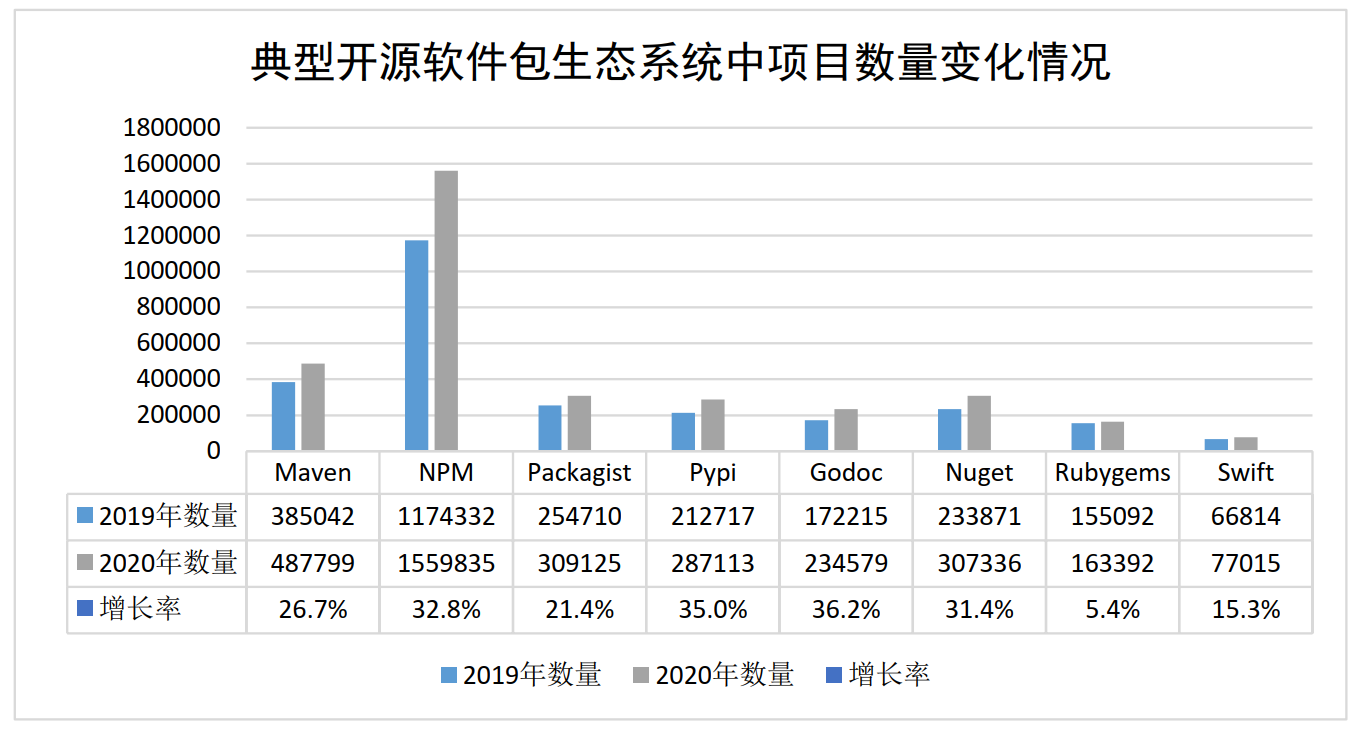
\includegraphics[width=12cm]{qianxin.png} \\
  \caption{2019和2020年八个典型开源软件包生态系统的增长情况}
 \label{fig:qianxin}
\end{figure}

\section{软件供应链安全}
软件供应链的上游软件可能悄无声息地影响着下游产品。开源软件之间的依赖关系错综复杂,在开发过程中,开发者通常借助包管理程序实现自动管理,因此可能意识不到产品中包含里数量巨大的开源软件。一旦某个上游的开源软件被发现安全漏洞,软件开发者无法立即意识到漏洞同时被引入到了产品中,隐含里巨大的软件供应链安全风险。

2020年5月,GitHub披露了Octopus Scanner漏洞\cite{octopus},该漏洞是针对Apache NetBeans IDE项目的开源软件供应链攻击,影响到了26个开源项目。

2020 年 12 月,安全公司FireEye发现全球著名的网络安全管理软件供应商 SolarWinds遭遇国家级 APT 团伙高度复杂的供应链攻击。该攻击在SolarWinds的一个数字签名组件DLL中插入后门,该后门通过HTTP协议与第三方服务器通信。

\section{安卓软件的供应链安全}
Appbrain\cite{appbrain}追踪了450个流行的库,统计结果显示它们在安卓生态系统中有着广泛的使用,广告库、社交网络库、以及手机设备分析库尤为受欢迎。如此广泛的第三方库使用在加速开发过程、避免重复造轮子的同时,也吸引着攻击者将目标向软件供应链上游移动,通过利用受欢迎的库的漏洞来达到攻击应用的目的。atvhunter 2-4。来自Trend Micro的安全研究团队披露百度提供的SDK中的Moplus包含的功能可能被恶意使用,以向用户设备植入后门\cite{baidu}。这一处于软件供应链上游的漏洞已经流入超过14000款安卓APP,可能使得约1亿用户处于黑客的攻击风险中。

2022年4月Google Play商店内的安卓应用超过260万,3月与4月新增应用数量均在2万左右,来自其他市场的应用更是不计其数。

如此数量的APP包含着不可忽视的供应链风险,但是由于APP包含着敏感信息或者具有商业价值的运行逻辑,大部分开发者基于安全和产权的考虑都会将产品进行混淆后再发布。这导致在对APP进行安全性检查时更加困难,识别混淆APP中引入的上游软件成为了亟待解决的问题。事实上,约78\%的漏洞都是在间接的依赖中找到,可能带来的安全风险则更加难以发现\cite{qianxin.com}。






\chapter{研究现状}

\section{检测混淆库}
随着APP混淆技术的成熟,以第三方库能够被容易地区分为前提的方法已不适用,标识符被混淆为无意义的简短的字母组合,比如\textit{com.google}可能被混淆为\textit{a.c},无法提供关于库的任何信息。图\ref{fig:hunxiao}为一个代码混淆的示例,仅从名称无法获得任何关于包的信息。

\begin{figure}[!htp]
  \centering
  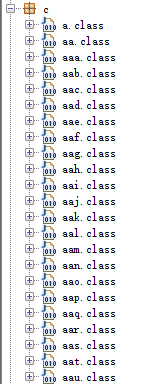
\includegraphics[width=3cm]{hunxiao.png} \\
  \caption{一款360软件的apk解压后得到的经过重命名混淆的class文件}
 \label{fig:hunxiao}
\end{figure}

T. Book等人的工作通过白名单的方法检测APP内的第三方库\cite{book2013longitudinal},但这类方法显然无法解决标识符重命名的问题。PEDAL\cite{liu2015efficient}借助机器学习方法,从SDK中提取代码特征,并使用包之间的关系信息训练了分类器来识别第三方库。


\section{检测未知库}

一些研究工作提出了在没有已知第三方代码的数据库知识情况下检测APP组成成分的方法。此类方法通常首先把开发者代码与第三方代码进行分类,再将第三方代码聚类成不同的组件,组件即一个可能的库的候选,进一步评估候选之间的相似度,当超过相似度阈值的候选的出现次数足够多时就认为找到了一个库。

如Chen等人\cite{chen2016following}从大量的APP中获取库,进行聚类和检测然而这一方法在混淆的情况下表现不佳,因为其假设不同APP中包含的库的相同实例拥有相同的包名,混淆打破了这一基本的假设。

为解决包名混淆问题,LibRadar\cite{ma2016libradar}使用特征哈希的方法,不需要基于包名的聚类,而是借助包中的目录结构来识别库的候选,具体来说是将一个候选表示为一个目录树的结构。这引入一个新的假设,即包的结构在混淆过程中不改变。但混淆工具可以将不同的包合并为一个包,很容易打破这一假设。

WuKong\cite{wang2015wukong}和AnDarwin\cite{crussell2014andarwin}用控制流图和API数量来定义哈希特征,用来计算各候选库的相似度。考虑到混淆工具可能修改一个方法的控制流图,或者移除在APP运行中未真正使用的方法,哈希的质量影响着这两类方法的表现性能。


\section{检测已知库}

基于已知库的检测要求关于现存库的知识,如库的基本信息、哈希特征等,在混淆APP第三方库识别的场景下,用构建知识数据库的代价换取了更好的表现。

具有代表性的一个工具是LibScout\cite{backes2016reliable},用包的结构以及类的哈希作为特征,进行APP与数据库中第三方库的匹配,在控制流篡改和包/类/描述符重命名情况下依然有效。但是随着数据库中的标准库代码特征增多,哈希特征的计算也应当考虑更多信息,导致特征生成时间与匹配时间增加。



\section{检测标准库的版本}

现有工作中以版本为目标实现精确检测的并不多,AdDetect\cite{narayanan2014addetect}仅能够区分广告和非广告的库,基于聚类的方法如LibRadar\cite{ma2016libradar},LibD\cite{li2017libd}等都没有声明能够检测库的特定版本。

实现版本的检测仍面临着很多问题:
\begin{enumerate}
\item{需要处理庞大的数据集。第三方库本身就纷繁复杂,如果再将各个版本考虑进去,将导致需要处理的数据成倍增长。}
\item{缺乏精确的表示。一个库的不同版本可能差异微小,如何找到合适的特征来区分这一差别非常关键。}
\item{代码混淆的干扰。代码混淆同样会导致库的代码发生改变,这种改变是由不同库引起还是由同一库的不同版本引起,需要被准确的区分。}
\end{enumerate}



\chapter{研究方法}

在参考了多篇文献后,我提出了一种适用于包的结构混淆、包/类/标识符重命名场景的,基于已知标准库的数据库,利用两类信息生成粗粒度/细粒度两级哈希特征的安卓应用第三方库及其特定版本的检测方法。



\section{方法概述}

此方法不依赖于包中的目录结构以及各级名称,因此可以抵抗结构混淆以及重命名混淆,包括了四个步骤:
\begin{enumerate}
\item{预处理jar、aar和apk。将来自Maven仓库的jar包、aar包以及待检测apk处理成便于构建树结构的形式。}
\item{构建特征树。根据上一阶段输出,将每个包作为根节点构建特征树,该包内的所有类,不论是根包的类还是子包的类,一律作为树的中间层节点,各类的方法作为叶子节点。特征分为粗粒度、细粒度两级特征。粗粒度特征为方法的描述符的返回值以及参数类型,细粒度特征为该方法的字节码,首先生成叶子节点的两级特征,再利用叶子节点生成中间层节点即类节点的特征。}
\item{构建数据库与匹配。根据以上特征生成方法,计算Maven仓库中的标准库的特征,并存储到数据库中。对待检测APP,首先生成粗粒度特征,确定所包含的库,再根据细粒度特征,确定各库的具体版本。}
\end{enumerate}



\section{包的预处理}

\subsection{Dex与Class文件的处理}

\subsubsection{Dex与Class简介}

\textbf{DEX文件:}DEX文件时Android系统中的一种文件,是一种特殊的数据格式,能够被Dalvik虚拟机识别并加载执行,类似于Windows上的EXE可执行文件。将APK安装包解压后得到的文件就包含了DEX文件,它记载了应用程序的全部操作指令以及运行时数据。当java程序编译成class文件后,还需要使用dx工具将所有的class文件整合到一个DEX文件里,目的是其中各个类能够共享数据,在一定程度上降低了冗余,同时也使文件结构更加紧凑。DEX文件大小通常是传统jar包的50\%左右。


\textbf{CLASS文件:}class文件是能够被java虚拟机识别,加载并执行的文件格式,通过javac程序可以从java源文件生成class文件。class文件记录了一个类文件的所有信息,不仅包含了java源代码中的信息,还包括了this、super等关键字的信息。作为一种8位字节的二进制六文件,class中的数据按顺序紧密排列,没有间隙,从而让JVM加载更加迅速,每一个类、接口或者枚举都单独占据一个class文件。


\subsubsection{Apk与jar的预处理}

预处理流程如图\ref{fig:preprocess}所示。
\begin{figure}[!htp]
  \centering
  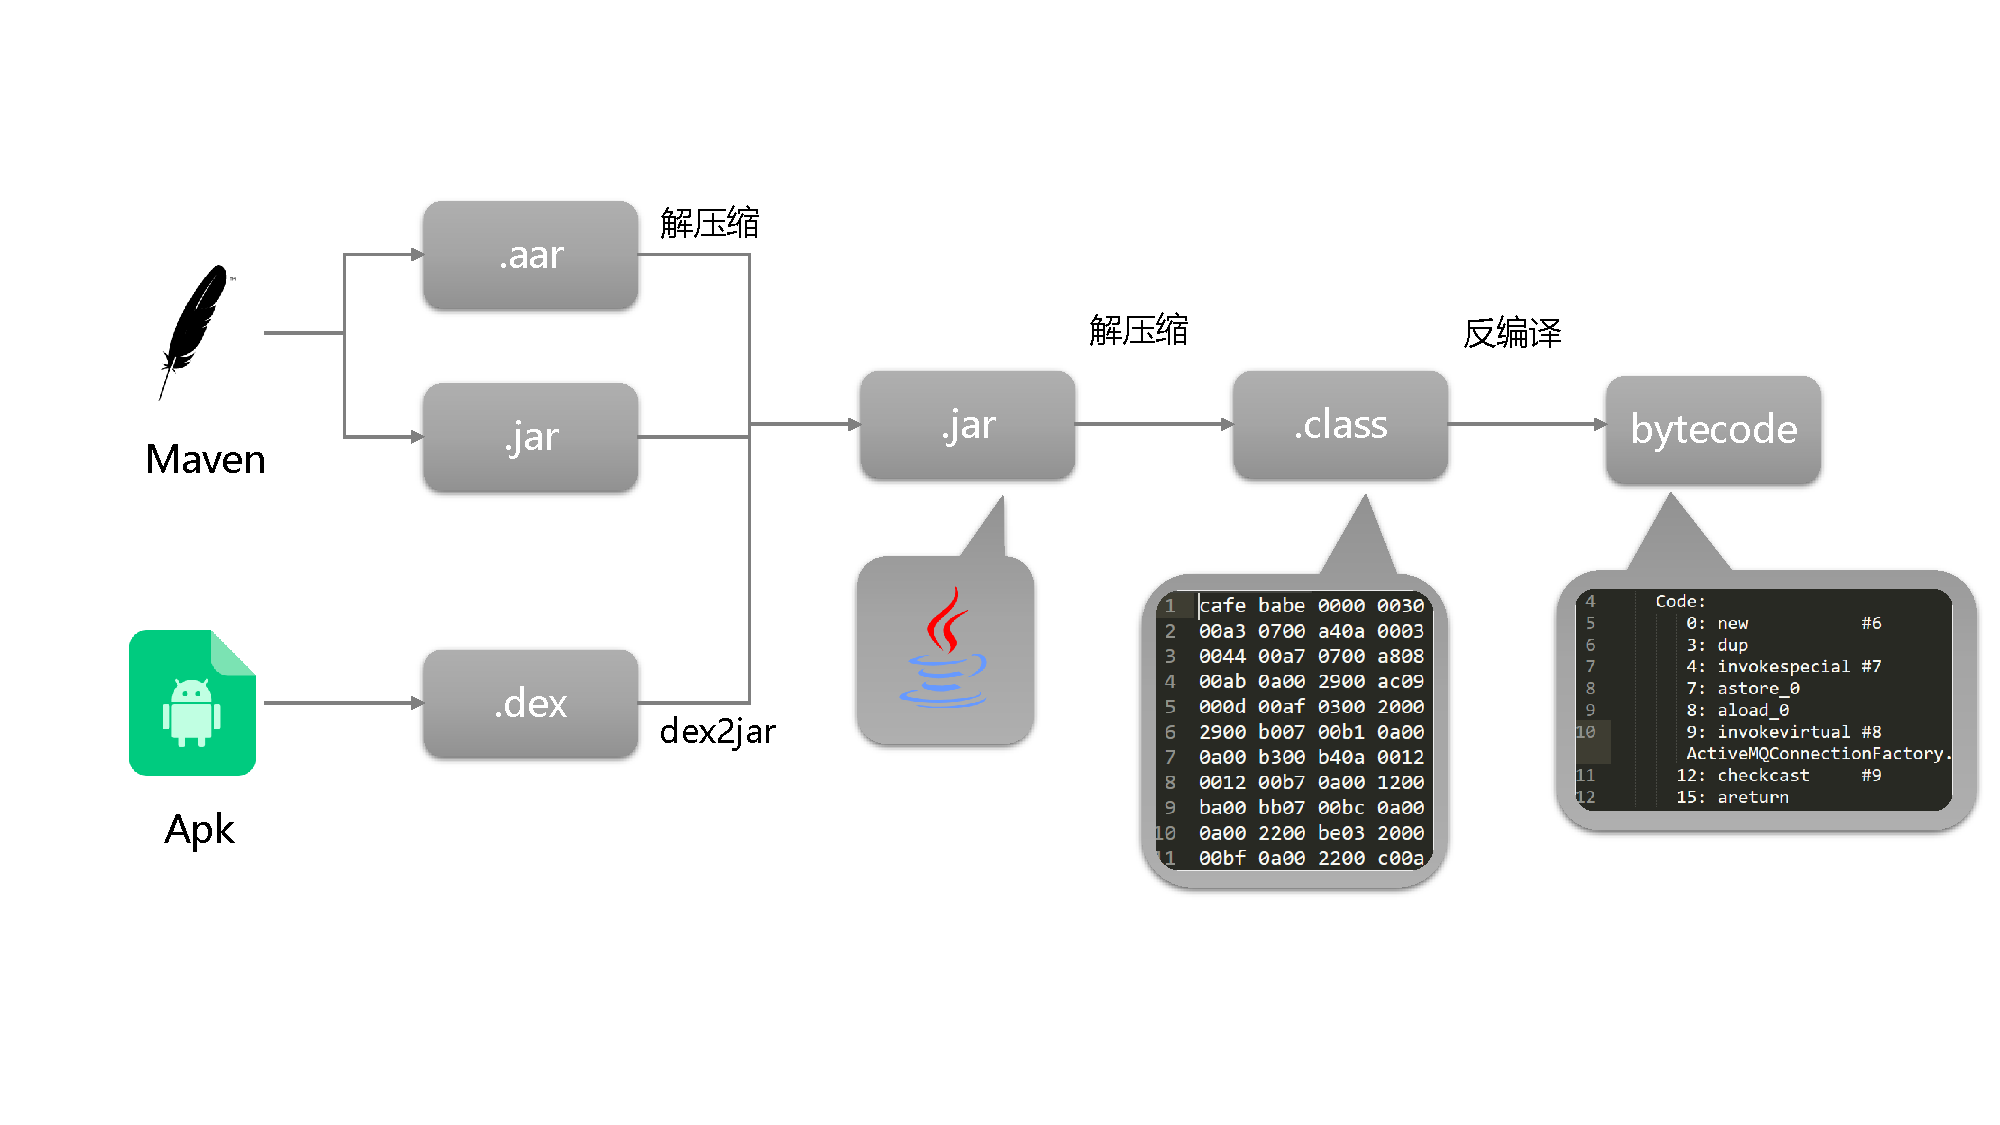
\includegraphics[width=15cm]{preprocess.pdf} \\
  \caption{Apk与标准库转换到java字节码的预处理流程}
 \label{fig:preprocess}
\end{figure}

\textbf{Apk预处理:}从应用市场获取待检测的应用的安装包,即apk文件。Apk文件本质上为zip格式的压缩文件,解压后可以得到dex文件。借助dex到jar的转换工具dex2jar\cite{d2j}将DEX文件转换为包含多个class文件。此处的class文件通常是经过软件开发者混淆的,大部分类的名称和函数的名称经过了混淆处理,不能提供有效信息,转换得到的包的目录结构也不可靠。


\textbf{Jar预处理:}Maven社区提供的中央仓库\cite{maven}包含了大量常用的库,包括绝大多数流行的Java开源构件,源码,许可证信息等,一般来说简单的Java项目依赖的构建都可以满足,因此选择Maven仓库中的部分jar包作为构建数据库的基础。我利用爬虫从Maven中央仓库中获取了大量的jar包或aar包,aar包需要先解压一次获得其中的jar包,将jar包解压就可以获得该标准库的各个class文件。在爬取标准库的过程中,需要跳过一些带有javadoc或者sources字样的链接,这表示该包为一个说明文档包或者源代码包,在此次工作中用不到。


\textbf{字节码的生成:}Java字节码是一种程序的低级表示,能够直接被java虚拟机所理解和翻译,以实现java跨平台的特性。具有二进制格式的class文件,实质上就是java的字节码,属于独立于平台和操作系统的指令集。为了删除class文件中的常量信息,我使用javap程序将class文件反编译为具有可读性的助记符形式的字节码,可以清楚地区分开描述符,代码,常量池等部分,并存储为文本文件供后续使用。




\section{构建特征树}

\subsection{两级特征}
如果特征的计算方法过于复杂,将会导致在获取apk特征时用时过长,因此本方法中采用了两级特征——粗粒度特征与细粒度特征,来解决这一问题,同时实现第三方库的版本检测。粗粒度特征计算方法简短、生成速度快、相应的精准度有所下降,用于确定待测apk中的包是数据库中的哪一个标准库。细粒度特征计算方法复杂、生成速度慢、但可以精确到单条字节码操作指令的层面。对于细粒度特征而言,即便同一个库的版本不同所导致的细微代码差异也能够体现出来,因此可以在包成功匹配的情况下进一步匹配具体版本。


\subsubsection{粗粒度特征}

粗粒度特征由函数的描述符生成,由于函数描述符包含了函数名、参数名,极易受到重命名混淆影响,因此我将名称部分删去,以\textit{返回值类型 (参数1类型,参数2类型,...,参数n类型)}的字符串作为描述符,计算其md5哈希值,得到该方法的签名,一个例子如表\ref{tab:descriptor}所示。尽管此签名可能在多个包中,乃至一个包中的不同类中出现,但是结合该类下的各个方法的签名,方法的序列,可以减少碰撞的概率,用于初步表示一个类。如表\ref{tab:activemq}所示,标准库\textit{org.codehaus.avtivemq}的两个类\textit{ActiveMQMessageConsumer}和\textit{BrokerClientImpl}在方法“\textit{public java.lang.String toString()}”上发生了碰撞,但是在其他方法上有很大差异,方法的总数也不同,从而类的层面的特征有所区别。


\begin{table}[!hpt]
  \caption{方法描述符的处理}
  \label{tab:descriptor}
  \centering
  \begin{tabular}{cp{8cm}} \toprule
%    \multicolumn{2}{c}{Item} \\ \cmidrule(r){1-2}
    原始描述符 & public static ActiveMQConnection makeConnection(String user, String password, String uri)\\ \midrule
    删除名称后的描述符  & public static org.codehaus.activemq.ActiveMQConnection makeConnection(java.lang.String, java.lang.String, java.lang.String) \\ \midrule
    md5哈希值      & befc542005082b1940176d89035826ab \\ \bottomrule
  \end{tabular}
\end{table}

\begin{table}[!hpt]
  \caption{标准库org.codehaus.activemq中的两个类包含方法(部分)的情况}
  \label{tab:activemq}
  \centering
  \begin{tabular}{ccc} \toprule
%    \multicolumn{2}{c}{Item} \\ \cmidrule(r){1-2}
    描述符 & ActiveMQMessageConsumer & BrokerClientImpl \\ \midrule
     public java.lang.String toString(); & \ding{51}  & \ding{55} \\ 
     protected long getStartTime(); & \ding{51} & \ding{55} \\
      protected void setBrowser(boolean); & \ding{51} & \ding{55} \\
    public void updateBrokerCapacity(int); & \ding{55} & \ding{51}\\ \bottomrule
  \end{tabular}
\end{table}



\subsubsection{细粒度特征}

细粒度特征基于函数的字节码生成。\textit{ActiveMQConnection}类的一个方法\textit{makeConnection}的字节码如下所示:

\begin{codeblock}[language=C]
  public static org.codehaus.activemq.ActiveMQConnection makeConnection(
  java.lang.String) throws javax.jms.JMSException;
    Code:
       0: new           #6                
       3: dup
       4: aload_0
       5: invokespecial #10                
       8: astore_1
       9: aload_1
      10: invokevirtual #8                
      13: checkcast     #9                
      16: areturn
\end{codeblock}


Java字节码是基于堆栈结构的,上面字节码“Code”部分的每一行对应于一条操作指令,仅仅表示对堆栈的操作,而不包含操作数。源代码中所定义的常量、变量名等静态成员存放在常量池中,因而避免了名称混淆的问题。每一条操作指令对应于一个十六进制的操作码,表\ref{tab:bytecode}展示了部分对应关系及其说明。


\begin{table}[!hpt]
  \caption{Java字节码助记符与十六进制操作码对应关系(部分)}
  \label{tab:bytecode}
  \centering
  \begin{tabular}{ccc} \toprule
%    \multicolumn{2}{c}{Item} \\ \cmidrule(r){1-2}
    助记符 & 操作码 & 说明 \\ \midrule
    new  & 0xbb & 创建一个对象,并将其引用值压入栈顶 \\
	dup & 0x59 & 复制栈顶数值,并将复制值压入栈顶 \\
	aload\_0 & 0x2a & 将第一个引用类型本地变量推送至栈顶 \\
	invokespecial & 0xb7 & 调用超类构造方法,实例初始化方法,私有方法 \\
	astore\_1 & 0x4c & 将栈顶引用型数值存入第二个本地变量 \\
	aload\_1 & 0x2b & 将第一个引用类型本地变量推送至栈顶 \\
	invokevirtual & 0xb6 & 调用实例方法 \\
	checkcast & 0xc0 & 检验类型转换,检验未通过将抛出异常 \\
	areturn & 0xb0 & 从当前方法返回对象引用 \\ \bottomrule
  \end{tabular}
\end{table}




\subsection{特征树的实现}

\subsubsection{字节码特征提取}

如图\ref{fig:tree}所示,字节码解析器布置在树的下方,其接收字节码文件,从文件头开始读入,利用正则表达式匹配每一个函数的描述符。当匹配成功时,表明一个函数的读入即将开始,则解析器依次读取函数描述符和操作指令序列,并将原始特征记录为一个特征对。当读至文件尾时,该class文件代表的类的所有成员函数全部读取完毕,将各特征对传递给上方的树。


\subsubsection{方法层}

方法实现为\textit{mNode}(Method Node)类。根据提取出来的字节码的原始特征,对于每一对粗/细粒度原始特征,生成一个方法节点,对原始特征进行处理。方法节点记录了原始的函数描述符,文件路径等基本信息,同时生成了处理后的特征的MD5哈希值,作为此方法的两级特征。表为\textit{ActiveMQConnection}类中方法\textit{createSession}的各个属性值。

\begin{figure}[!htp]
  \centering
  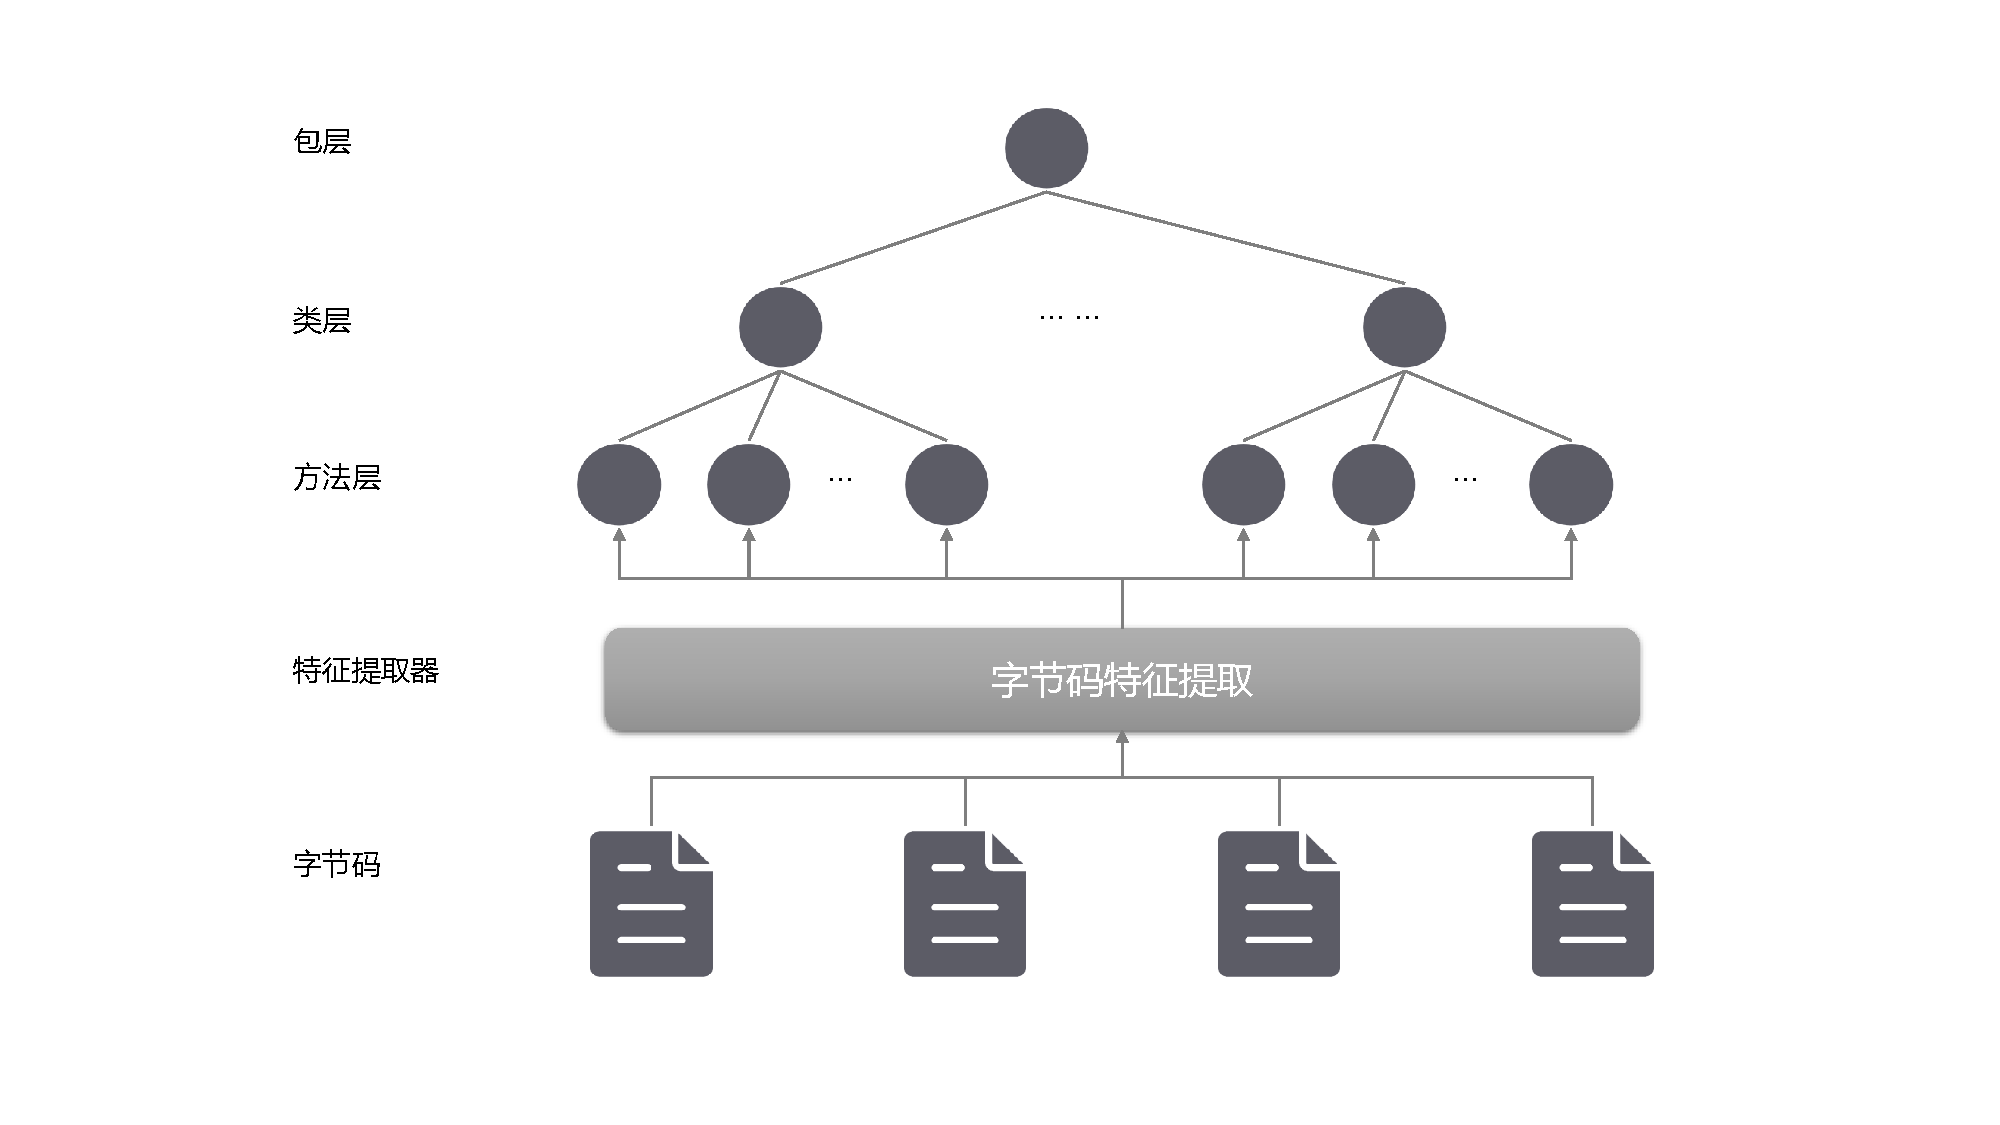
\includegraphics[width=15cm]{tree.pdf} \\
  \caption{使用特征提取器从字节码文件中获取特征并存储为树型数据结构}
 \label{fig:tree}
\end{figure}

\subsubsection{类层}

类实现为\textit{cNode}(Class Node)类,类层根据该class文件中包含的方法,将各个方法对应的\textit{mNode}节点作为自己的子节点。不同类的方法数大相径庭,有的类没有方法,只有数据成员,有的类则包含几十甚至上百个函数成员。再考虑到类的不同版本之间可能差异很小,仅仅体现在个别方法的几个函数上,类的特征必须能体现函数成员的特征。因此我采用了模糊哈希的方法,算法如\ref{algo:fuzzyhash}所示,将类下各方法的特征进行排序、连接,计算模糊哈希值作为类的粗/细粒度特征。

此处模糊哈希的用法与ATVHunter\cite{zhan2021atvhunter}有相似之处,都是为了降低代码混淆对最后特征带来的影响,但是ATVHunter的目标是减少部分指令改变对函数签名的影响,而此处是减少部分函数改变对类的特征的影响。如图\ref{fig:fuzzy}所示,模糊哈希的应用步骤为:
\begin{enumerate}
\item{将类下各方法的特征连接成一个序列。}
\item{使用滑动窗口(滚动哈希)将序列分割成不同的切片。}
\item{对每个切片,计算其MD5哈希值,取最后6位作为压缩映射值。}
\item{最后将所有映射值连接起来作为最终值。}
\end{enumerate}

\begin{figure}[!htp]
  \centering
  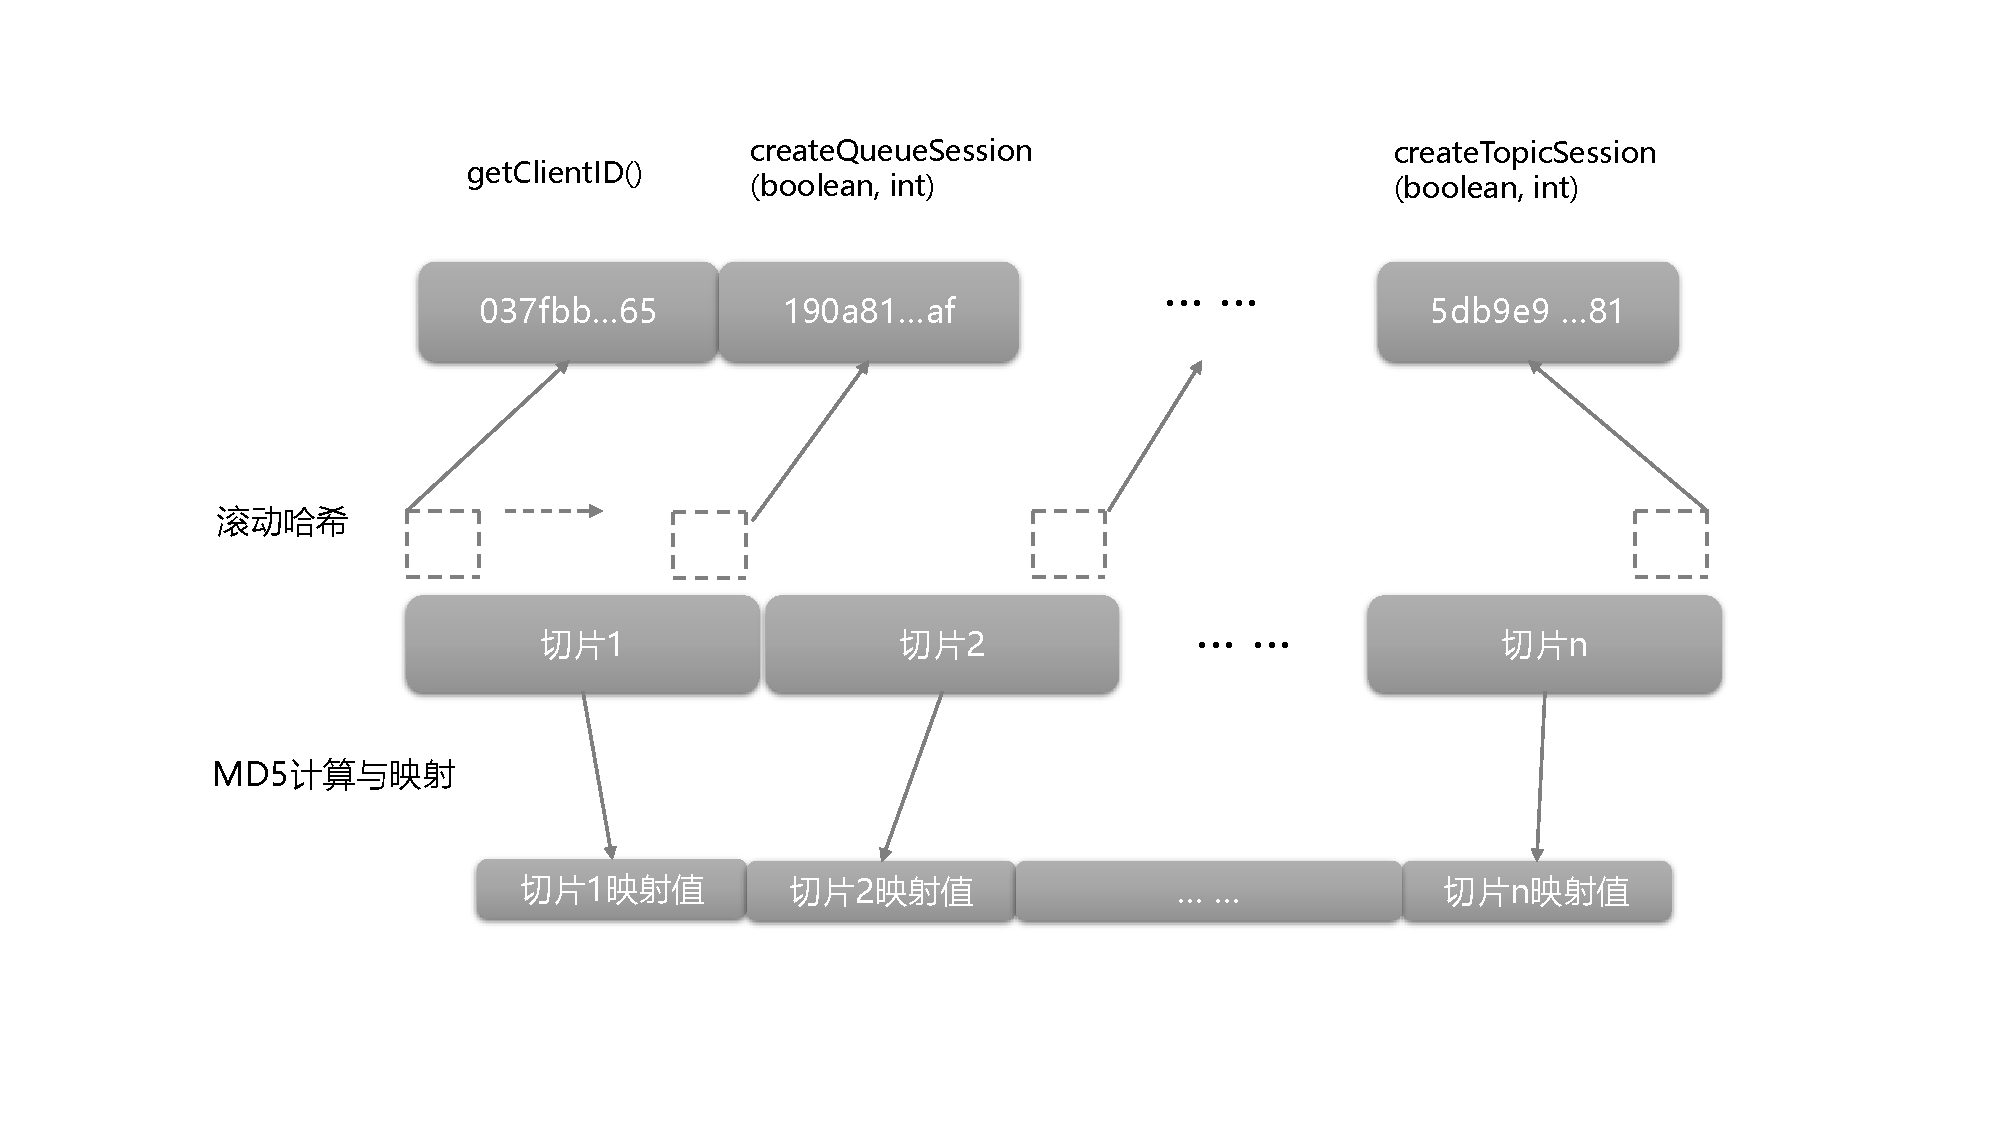
\includegraphics[width=15cm]{fuzzy.pdf} \\
  \caption{使用特征提取器从字节码文件中获取特征并存储为树型数据结构}
 \label{fig:fuzzy}
\end{figure}



\begin{table}[!hpt]
  \caption{标准库org.codehaus.activemq中的两个类包含方法(部分)的情况}
  \label{tab:activemq}
  \centering
  \begin{tabular}{cc} \toprule
%    \multicolumn{2}{c}{Item} \\ \cmidrule(r){1-2}
    方法 & org.codehaus.activemq.ActiveMQConnection\$createSession  \\ \midrule
    描述符特征 & public javax.jms.Session(boolean, int)  \\ 
    字节码指令序列 & 2a b6 2a b6 bb 59 2a 1b 99 03 a7 1c b7 b0 \\
    粗粒度特征 & d8a58a75cf9b3272e8736cd74256fdc7 \\
    细粒度特征 &  45422e23d690d166bc6dd144f226076f \\ \bottomrule
  \end{tabular}
\end{table}


\begin{algorithm}[htb]
  \caption{类的模糊哈希值计算}
  \label{algo:fuzzyhash}
  \small
  \SetAlgoLined
  \KwData{类节点cNode}
  \KwResult{类的模糊哈希值Fuzzy\_hash }

  initialization\;
  sort(cNode.getMethods())\;
  Sequence$\leftarrow$null\;
  \For{mNode $\in$ cNode.getMethods()}{Sequence $\leftarrow$ Sequence $cascade$ mNode.getFeature()\;}
  Slices$\leftarrow$rolling\_hash(Sequence)\;
  Fuzzy\_hash$\leftarrow$null\;
  \For {slice $\in$ Slices}{F\_hash\_slice$\leftarrow$mapping\_function(MD5(slice))\;
  					 Fuzzy\_hash$\leftarrow$Fuzzy\_hash $cascade$ F\_hash\_slice\;}

\end{algorithm}


\subsubsection{包层}

包实现为\textit{pNode}(Package Node)类,是一个特征树的根节点。包层不产生特征,用于管理属于该包下的各个类。为了解决APK产生的包中可能存在目录结构的混淆问题,每一个包都采用根包作为唯一的根节点,其下包含的子包以及子包中的二级子包等所拥有的类都归为根包的类。

最后将从包到方法的各个节点封装为一个\textit{javaTree}类,负责统筹管理从文件的筛选到各级节点的生成等诸多工作。



\subsection{特征存储}

为了便于特征的查找与管理,我将哈希树输出的特征存放在MySQL数据库中,步骤如下:

\begin{enumerate}
\item{设计数据库scheme:tpl如表\ref{tab:mysql}所示,在tpl下创建表maven,存储从Maven仓库获取的标准库。}
\item{遍历本地爬取到的Maven仓库,当文件夹中包含\textit{META-INF}时表明当前目录为一个根包的目录。}
\item{在根包的目录上构建哈希树,解析目录中的文件,形成该包下各类、各方法的特征。}
\item{用插入语句将特征存储到数据库中}
\end{enumerate}

\begin{table}[!hpt]
  \caption{MySQL数据库中tpl的scheme}
  \label{tab:mysql}
  \centering
  \begin{tabular}{l|lllll} \toprule
%    \multicolumn{2}{c}{Item} \\ \cmidrule(r){1-2}
    字段 &  package & class & method & coarse feature & fine feature \\ \midrule
    数据类型 & varchar(255) & varchar(255) & varchar(1024) & varchar(255) & varchar(255)  \\  \bottomrule

  \end{tabular}
\end{table}



\subsection{特征匹配}


\begin{table}[!hpt]
  \caption{标准库与安卓应用的相关符号及说明}
  \label{tab:symbol}
  \centering
  \begin{tabular}{cc} \toprule
%    \multicolumn{2}{c}{Item} \\ \cmidrule(r){1-2}
    符号 &  说明 \\ \midrule
    $T_{sim}$ & 相似度阈值,相似度超过此值的两个特征认为互相匹配 \\
	$feature_{lib}$ & 来源于标准库的一个类或者方法的特征 \\ 
	$feature_{app}$ & 来源于安卓应用的一个类或者方法的特征 \\
	$C_{lib}$ & 标准库所包含的类的集合 \\
	$C_{app}$ & 安卓应用所包含的类的集合 \\
	$M_{class}$ & 类所包含的方法的集合\\
	$Similarity_p$ & 两个包之间的相似度\\
	$Similarity_c$ & 两个类之间的相似度\\
	 \bottomrule

  \end{tabular}
\end{table}


\subsubsection{相似度}

为了表征标准库与来自Apk的包的相似程度,我引入了相似度来量化这一概念。相似度适用于不同来源(Maven/APP)的类或方法的匹配,是一个介于0和1之间的数,1表示完全匹配。若要判断APP所包含的包是否存在于数据库中,需要查看数据库中是否存在足够数量的类,使得这些类的特征值与APP中类的特征值的相似度都超过了一定阈值。由于类的特征值是根据方法的特征值生成的,因此类的相似程度能过说明其内各个方法的相似程度。类和方法的特征均为字符串序列表示的哈希值,因此用编辑距离来计算两个序列之间的相似度:
\begin{equation}
Similarity(feature_{lib},feature_{app})=\frac{edit\_distance(feature_{lib},feature_{app})}{max\{length(feature_{lib}),length(feature_{app})\}}
\end{equation}

对于待定的阈值$T_{sim}$,定义来自标准库的特征$feature_{lib}$与来自APP的特征$feature_{app}$匹配,如果满足:

\begin{equation}
Similarity(feature_{lib},feature{app})\ge T_{sim}
\end{equation}


同时,标准库的规模也应该纳入考虑范畴。一些大规模的类、或者相似的类,可能在部分方法上有相似之处,在实现逻辑上有相同点,因此不能仅仅因为成功匹配其下的一部分类就将其所谓候选库。而一些小规模的类,方法数可能很少,一定数量的类匹配就说明其有很大概率就是APP所使用到的库。一种简明的相似度计算方法如下:
\begin{equation}
Similarity_p(lib,app)=\frac{|\{c_1,c_2,\dots ,c_n\}|}{|C_{lib}|} \in [0,1]
\end{equation}

其中,$c_i$满足:
\begin{subequations}
\begin{align}
(a)&\ c_i \in C_{lib}\\
(b)&\ \exists\  c'\in C_{app},Similarity(c_i,c')\ge T_{sim}
\end{align}
\end{subequations}


类似地,用$Similarity_c$表示方法相似度,也可以在方法粒度上实现更为精确的匹配:
\begin{equation}
Similarity_c(class_{lib},calss_{app})=\frac{|\{m_1,m_2,\dots ,m_n\}|}{|M_{class_{lib}}|} \in [0,1]
\end{equation}

其中,$m_i$满足:
\begin{subequations}
\begin{align}
(a)&\ m_i \in M_{class_{lib}}\\
(b)&\ \exists\  c'\in M_{class_{app}},Similarity(m_i,m')\ge T_{sim}'
\end{align}
\end{subequations}



